\documentclass{article}
\usepackage[latin1]{inputenc}
\usepackage[spanish,es-tabla]{babel}
\usepackage{amsmath}
\usepackage{helvet}
\usepackage{caption}
\usepackage{graphicx}
\captionsetup{labelsep=period}
\captionsetup[table]{skip=1pt}
\spanishdecimal{.}
\begin{document}

\section{Revisi�n de columna de concreto}
Revisi�n de columna de concreto a flexo compresi�n

%% Datos iniciales
\subsection{Datos de los elementos}

Los datos de  la columna se muestran en la tabla \ref{t:datos}

\begin{table}[htbp]
\caption{Datos de la columna}
\label{t:datos}
\centering
\begin{tabular}{|llll|}
\hline
Dato & Valor & Unidades & Comentarios \\ \hline
b     & 20.00    & cm         & Ancho de la columna       \\ 
b     & 20.00    & cm         & Ancho de la columna       \\ 
r     & 3.00     & cm         & Recubrimiento              \\ 
f'c   & 250   & $kg/cm^2$  & Resistencia del concreto    \\ 
fy    & 4200  & $kg/cm^2$  & Resistencia del acero      \\ \hline 
\end{tabular}
\end{table}

\subsection{Compresi�n pura}

La resistencia a compresi�n pura se obtiene con:

\begin{equation}\label{eq:pu}
P_u=F_r(A_g f''_c + A_s f_y )
\end{equation}

donde $P_u$ es la capacidad resistente del concreto, $F_r=0.75$, $A_g$ es el �rea del concreto, $A_s$ es el �rea del acero.
El �rea del concreto se obtiene con $A_g=BH$; el �rea de una varilla del \#4 es 1.27 cm por lo que:
 
\begin{align*}
A_g=& (20.00)(20.00) \\ 
A_g=& 400.00 cm^2 \\ 
A_s=& 1.27(8) \\ 
A_s=& 10.13 cm^2 \\ 
\end{align*}

Por lo que el la resistencia a compresi�n pura es:

\begin{align*}P_u=&0.75[(400.00)(0.85)(250) + (10.13)(4200)]\\ 
P_u=&95672.57 kg 
\end{align*} 

\subsection{Flexo-Compresi�n}
Para el dise�o a flexo-compresi�n se propone un eje neutro $c$ a diferentes distancias para obtener su capacidad a flexi�n y compresi�n.

Para obtener la deformaci�n de cada barra de acero se considera que la deformaci�n act�a como se muestra en la Figura %\ref{fig:def}

Para obtener las deformaciones en cada punto se considera que la deformaci�n se obtiene con:

\begin{equation}\label{eq:def}
\epsilon_i=\left(\frac{d_i-c}{d-c}\right)0.003
\end{equation}

donde $\epsilon_i$ es la deformaci�n de la barra de acero a una altura $i$ deseada, $d_i$ es la distancia de la barra de acero $i$ a la barra m�s profunda, $d$ es el peralte efectivo, y $c$ es la distancia al eje neutro desde la barra m�s profunda.

En la Tabla \ref{t:di} se muestran las distancias $d_i$ de cada barra con sus respectivas �reas.

\begin{table}[htbp]
\caption{Distancias de cada barra respecto a la barra mas profunda}
\label{t:di}
\centering
\begin{tabular}{|lll|}
\hline
Barra & $d_i$(cm) & $A_s$($cm^2$) \\ \hline
1     & 14.00    & 3.80                 \\ 
 2     & 7.00    & 2.53                 \\ 
 3     & 0.00    & 3.80                 \\ 
 \hline
\end{tabular}
\end{table}

Considerando un eje neutro igual a $c=3.00$ y aplicando la ecuaci�n \ref{eq:def} se tiene que para la barra 1 la deformaci�n es: 
 
 \begin{align*}
\epsilon_1&=\left(\frac{14.00-3.00}{17.00-3.00}\right)0.003\\ 
\epsilon_1&=0.0024
\end{align*}

Aplicando las ecuaciones para las dem�s barras se tiene

\begin{align*}
\epsilon_2&=0.0009\\ 
\epsilon_3&=-0.0006\\ 
\end{align*}

El esfuerzo m�ximo que alcanza el acero es $\epsilon_s =0.002$ por lo que se considera la siguiente desigualdad

\begin{equation}\label{eq:fs}
F_s=\epsilon E_y \le 0.002 E_y
\end{equation}

Cosndierando que $E_y=2 100 000 kg/cm^2$ se tiene entonces que los esfuerzos de cada barra son:

\begin{align*}
Fs_1&=(0.0024)(2100000)&=&4200.00kg/cm^2 \\ 
Fs_2&=(0.0009)(2100000)&=&1800.00kg/cm^2 \\ 
Fs_3&=(-0.0006)(2100000)&=&-1350.00kg/cm^2 \\ 
\end{align*}

Para obtener la fuerza se multiplica el esfuerso $F_s$ por el �rea por lo que las fuerzas se muestran en la Tabla \ref{t:fuerzas}

Para obtener la fuerza a compresi�n del concreto se aplica la ecuaci�n \ref{eq:conC}

\begin{equation}\label{eq:conC}
F_c=(0.85)(f'c)(B)0.85(d-c)
\end{equation}

Por lo que la fuerza compresi�n del concreto es

\begin{align*}
F_c&=(0.85)(250)(20.00)0.85(17.00-3.00)\\ 
F_c&=50575.00 kg
\end{align*}

En la tabla \ref{t:fuerzas} se muestran las fuerzas del acero y concreto

\begin{table}[htbp]
\caption{Fuerzas de cada barra}
\label{t:fuerzas}
\centering
\begin{tabular}{|lllll|}
\hline
Barra  & $\epsilon$ & $F_s$($kg/cm^2$) & $A_s$($cm^2$)&$F_i$($kg$)\\ \hline
1     & 0.0024    & 4200.00 & 3.80 & 15961.29                \\
2     & 0.0009    & 1800.00 & 2.53 & 4560.37                \\
3     & -0.0006    & -1350.00 & 3.80 & -5130.41                \\
Concreto     & 0.003    &250&&50575.00                \\ \hline 
&&&$P_r$=&65966.24\\ \hline 

\end{tabular}
\end{table}

Para obtener los momentos se requiere multiplicar las fuerzas de la Tabla \ref{t:fuerzas} por su brazo de palanca al centro de la columna. 

El brazo de palanca para el bloque de concreto se obtiene:

\begin{equation}\label{eq:brazo}
b_r=\left[B-0.85(d-c)\right]/2
\end{equation}

por lo que el brazo de palanca es

\begin{align*}
b_r&=\left[20.00-0.85(17.00-3.00)\right]/2 \\ 
b_r&=4.05 cm 
\end{align*}

En la tabla \ref{t:momentos} se muestran los momentos del acero y concreto

\begin{table}[htbp]
\caption{Momentos}
\label{t:momentos}
\centering
\begin{tabular}{|llll|}
\hline
Barra  & Fuerza (kg) & Brazo (cm) & Momento (kg-cm) \\ \hline
1      & 15961.29      & 7.00    & 111729.00      \\ 
2      & 4560.37      & 0.00    & 0.00      \\ 
3      & -5130.41      & -7.00    & 35912.89      \\ 
Concreto      & 50575.00      & 4.05    & 204828.75      \\ \hline 
  &    &  Suma& 352470.64 T-m      \\ \hline
\end{tabular}
\end{table}


En la Figura \ref{fig:ConcreteCol} se muestra el diagrama de interacci�n de la columna

\begin{figure}[htbp]
	\centering
		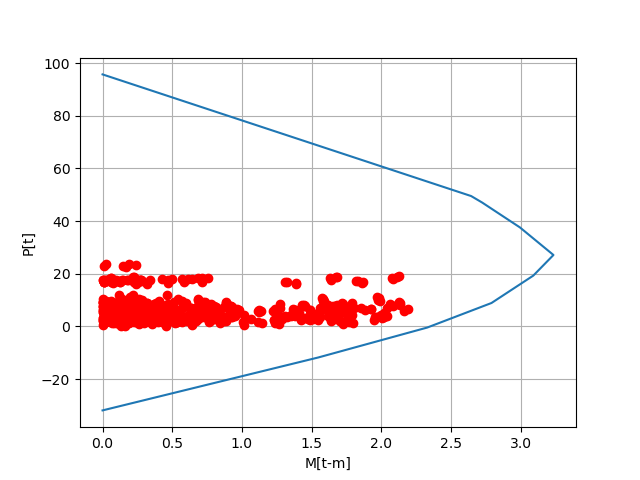
\includegraphics[width=0.80\textwidth]{D:/Investigacion/Latex/Latex/Ingenieria/Concreto/Columna/ColumnaConcreto/Python/ConcreteCol.png}
	\caption{Diagrama de Interacci�n de Columna}
	\label{fig:ConcreteCol}
\end{figure}

\end{document}
